\clearpage\section{Labs}\begin{Lab}

\begin{exe} {Verify system is ready for KVM }

   Verify the CPU chip extensions are available and enabled to support virtualization. 
   Confirm the required packages are available. 

   This exercise requires a 64 bit architecture system.

   It is common practice to run virtual machines as a non-root user, but in this
   exercise we will execute the commands as root.

   \begin{sol}
      \begin{enumerate}
         \item	Verify the cpu has virtualization support enabled.
		 \begin{raw}
# grep -e svm -e vmx /proc/cpuinfo 
		\end{raw} 
		      The output should have one of the flags highlighted, either 
		      \textbf{svm} or \textbf{vmx}. If no output was produced, verify 
		      in your \textbf{BIOS} that virtualization is supported. 
	\item install required packages:		      
         \begin{itemize}
            \item
            On \textbf{CentOS7}:
            \begin{raw}
# yum install qemu-kvm libvirt virt-manager virt-install virt-viewer 
	    \end{raw}
            \item
            On \textbf{OpenSUSE}:
            \begin{raw}
# zypper install qem-kvm libvirt virt-manager virt-viewer bridge-utils 
            \end{raw}
            \item
            On \textbf{Ubuntu}:
            \begin{raw}
# apt-get install qemu-kvm libvirt-bin virtinst \
		    virt-manager libosinfo-bin virt-viewer 
            \end{raw}
         \end{itemize}

         \item
         Verify and optionally start and enable the \textbf{libvirtd} service.

         \begin{raw}
# systemctl status libvirtd
# systemctl start libvirtd
# systemctl enable libvirtd
# systemctl status libvirtd
         \end{raw}

 	\item 
	If using \textbf{Ubuntu} or \textbf{Centos} please log in 
		      with \textbf{GNOME Xorg} not \textbf{GNOME Wayland}.
	\item 
	If using \textbf{openSUSE} you may have to add 
		      \textbf{export LIBVIRT\_DEFAULT\_URI=qemu:///system} \\
		      to 
		      \filelink{/etc/bash.bashrc.local}.  
		      
		      This will allow a regular user 
		      to administer all the virtual machines. 
		      \begin{raw}
# echo "export LIBVIRT_DEFAULT_URI=qemu:///system"  >> /etc/bash.bashrc.local
			\end{raw}
	\item 
	If challenged for the administrator password using \textbf{virsh} commands 
		      similar to the following screenshot.


\begin{figure}[H]
      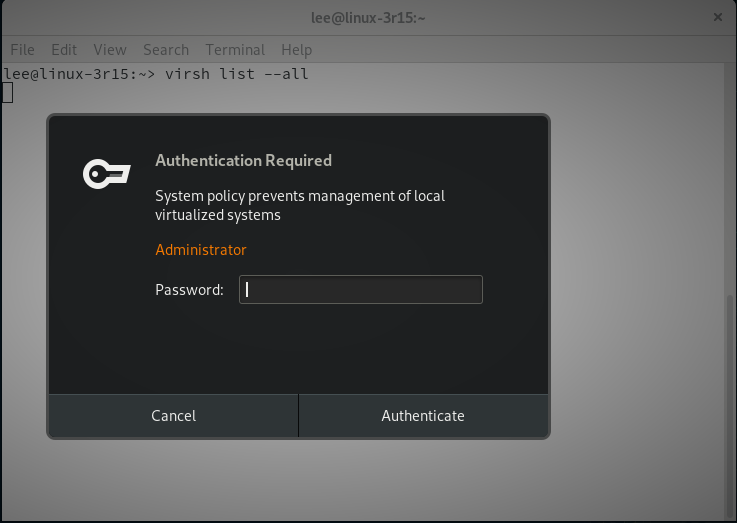
\includegraphics[height=3.2in]{IMAGES/libvirt-auth.png}
      \caption{libvirt authentication prompt}
   \end{figure}



	Set the \textbf{unix\_sock\_group} variable in \filelink{/etc/libvirt/libvirtd.conf}
		      to \textbf{libvirt}, it may be added to the bottom of the file like:
		      \begin{raw}
# echo 'unix_sock_group = "libvirt" ' >> /etc/libvirt/libvirtd.conf
			\end{raw}
			Then add the additional supplemental group \textbf{libvirt} group to your user:
			\begin{raw}
# usermod -a -G libvirt <username> 
			\end{raw} 

      \end{enumerate}

   \end{sol}

\end{exe}

\begin{exe} {Create and run a Virtual Machine based on an image}

	Often a virtual disk is used for distributing a pre-configured environment,
	this exercise will Create a virtual machine using an \textbf{xml} file as input to \textbf{virsh}.

	The parameters for the virtual machine are:
	\begin{itemize}
		\item name is \textbf{tiny2}
		\item 1 virtual CPU
		\item 512M memory
		\item the virtual disk is \file{/var/lib/libvirt/images/tiny2.vmdk}
		\item use \textbf{virt-viewer} to access the virtual machine
	\end{itemize}
	In this exercise a pre-installed disk \file{tiny2.vmdk} contains a 
	operating system and application to be made available. A \textbf{virsh}
	define command is 
	to be used with a \textbf{xml} configuration file. 

	\textbf{Note:} As an added extra credit adventure, some distro's 
	do not support writing to a \textbf{vmdk} image file. If \textbf{CentOS7}
	is being used for the host, the tiny2.vmdk must be converted to qcow2. The 
	conversion is done with the \textbf{qemu-img} command. 

	This will convert the file: 
		\begin{raw}
# qemu-img convert -O qcow2 tiny2.vmdk tiny2.qcow2 
		\end{raw}
	You will have to remember to adjust the file name in the rest of the lab exercise.

		
	\begin{sol}
	
		\begin{enumerate}
		\item Create a copy of the disk image and store it at \file{/var/lib/libvirt/images/tiny2.vmdk}
		\item Create an \textbf{xml} configuration file. 
			(a sample file is included in the
				\filelink{_SOLUTIONS} directory)

		\textbf{Note:} There are two sample files one 
			for \textbf{Ubuntu} called \filelink{tiny2.xml-ubuntu}
			and for \textbf{CentOS} called 
			\filelink{tiny2.xml-centos}, the difference is the 
			name of the \textbf{emulator} in the file, please 
			select the correct example file for your lab environment. 
			\rawfile{tiny2.html.inc}
		\item define the virtual machine 
			\begin{raw}
# virsh define tiny2.xml
			\end{raw}
		\item verify the configuration file 
			\begin{raw}
# virsh dumpxml tiny2 
			\end{raw}
		\item start the virtual machine 
			\begin{raw}
# virsh start tiny2
			\end{raw}
		\item connect to the virtual machine
			\begin{raw}
# virt-viewer tiny2 
			\end{raw}
		\item exit the virt-viewer and verify the state of the VM
			\begin{raw}
# virsh list --all 
			\end{raw}
		\item try a graceful shutdown of the VM, success or failure will depend on the OS
			\begin{raw}
# virsh shutdown tiny2 
			\end{raw}
		\item issue a forced shutdown of the VM if the graceful shutdown did not work
			\begin{raw}
# virsh destroy tiny2 
			\end{raw} 
		\end{enumerate}

	\end{sol}
\end{exe}

\begin{exe}  {Create a Virtual Machine using virt-install}

	
	In the previous exercise \textbf{virsh} 
	was used to create the configuration using an xml file as input.


	The object of this exercise is to simplify the install procedure 
	by using the \textbf{virt-install} tool. 

	One feature of \textbf{virt-install} is the 
	automatic configuration of a default network connection. 
	This feature can be overridden if desired. In this exercise the default 
	network connection will be used. 

	 The parameters for the virtual machine are:
        \begin{itemize}
                \item name is \textbf{tiny3}
                \item 1 virtual CPU
                \item 512M memory
                \item the virtual disk is \file{/var/lib/libvirt/images/tiny3.vmdk},
			a copy of the previously used \textbf{tiny2.vmdk}
		\item use a network connection called \textbf{default}
                \item use \textbf{virt-viewer} to access the virtual machine
	\end{itemize} 

	Once the \textbf{VM} has been created and tested that it runs, compare the active 
	configuration that \textbf{libvirt} has stored. The configuration created by
	\textbf{virt-install} will have many more default options enabled, including 
	an active network connection NAT'd to the default adapter on the host computer.

	\begin{sol}
		\begin{enumerate}
		\item  Create a copy of \textbf{tiny2.vmdk} and place it in
			\file{/var/lib/libvirt/images/tiny3.vmdk}
			\begin{raw}
# cp \file{/var/lib/libvirt/images/tiny2.vmdk} \file{/var/lib/libvirt/images/tiny3.vmdk}
			\end{raw}
		\item Confirm or create a user called \textbf{dnsmasq}, it is used by
			libvirt. 
		\begin{raw}
# grep dnsmasq /etc/passwd
		\end{raw} 
			if the user \textbf{dnsmasq}  does not exist, create it.
		\begin{raw}
# useradd dnsmasq
		\end{raw} 
		\item Verify a virtual network called \textbf{default} 
			exists and is set to autostart.
				\begin{raw}
# virsh net-list --all 
 Name                 State      Autostart     Persistent
----------------------------------------------------------

				\end{raw} 
			If the \textbf{default} network does not exist, use
				\textbf{virsh} to define the network from the xml
				file \filelink{default-net.xml}. 
				
				The contents of the 
				\filelink{default-net.xml} are: 
				\begin{raw}
<network>
  <name>default</name>
  <uuid>96ea6db6-cfb9-48fa-ad6a-bd21ab81c0d3</uuid>
  <forward mode='nat'>
    <nat>
      <port start='1024' end='65535'/>
    </nat>
  </forward>
  <bridge name='virbr0' stp='on' delay='0'/>
  <mac address='52:54:00:95:cb:bd'/>
  <domain name='default'/>
  <ip address='192.168.122.1' netmask='255.255.255.0'>
    <dhcp>
      <range start='192.168.122.128' end='192.168.122.254'/>
    </dhcp>
  </ip>
</network>
				\end{raw}

				Based on the default-net.xml file, the command to 
				define the network is:
				\begin{raw}
# virsh net-define default-net.xml 
Network default defined from default-net.xml
				\end{raw}
				Then set the network to autostart:
				\begin{raw}
# virsh net-autostart default 
Network default marked as autostarted
				\end{raw}
				Verify the network looks good. 
				\begin{raw}
# virsh net-list --all 
 Name                 State      Autostart     Persistent
----------------------------------------------------------
 default              inactive   yes           yes

				\end{raw}
				Start the new network. 
				\begin{raw}
# virsh net-start default
				\end{raw}

		\item  Use the virt-install command to \textbf{import} the existing 
			virtual machine's disk into a new configuration.
			\begin{raw} 
# virt-install \
              --name tiny3 \
              --memory 512 \
              --disk /var/lib/libvirt/images/tiny3.vmdk \
	      --os-type linux --os-variant generic  \
              --import
			\end{raw}
		
		\item 
			Examine the active configurations stored by \textbf{libvirt}. 
			\begin{raw}
# virsh dumpxml tiny3 > /tmp/tiny3.xml.dump
# virsh dumpxml tiny2 > /tmp/tiny2.xml.dump
			\end{raw} 

			Use commands like diff and ls to see the difference in the xml.dump files. 

		\end{enumerate}

	\end{sol}

\end{exe} 

\begin{exe} {Create a VM and install from a CD-rom image} 

	This exercise will demonstrate installation of an operating system from a CD-rom 
	using \textbf{virt-install}. 
	The CD-rom image is available in resources tar file installed earlier. Since 
	installation of operating systems can be long time and require access to 
	download updates or repository data a small self contained OS was chosen for 
	this exercise. 

	\textbf{Note:} During the initial start up, we will be overriding a default setting 
	and using a text mode console. This avoids some interesting issues with the mouse 
	during the installation of Tiny Core Linux. 

 The parameters for the virtual machine are:
        \begin{itemize}
                \item name is \textbf{tinycore}
                \item 1 virtual CPU
                \item 512M memory
		\item 0.1G new disk 
                \item the virtual disk is \file{/var/lib/libvirt/images/tinycore.qcow2}
                \item the virtual cd is \file{/var/lib/libvirt/images/CorePlus-current.iso}
                \item use \textbf{virt-viewer} to access the virtual machine
	\end{itemize}

	\begin{enumerate}
	\item Verify the CD-rom image is in the directory specified.
		\begin{raw}
# ls -l /var/lib/libvirt/images 
		\end{raw}
	\item Boot from the CD-rom using \textbf{virt-install} using the options specified below:
		\begin{raw}
# virt-install  --name tinycore --memory 512 --vcpus 1 \
		--cdrom /var/lib/libvirt/images/CorePlus-current.iso \
		--disk /var/lib/libvirt/images/tinycore.qcow2,size=0.1 \
		--os-type linux --os-variant generic --boot useserial=on 
		\end{raw}
			A \textbf{virt-viewer} window should pop open. 
		\item When the initial Core Plus screen appears, press the \textbf{tab} key. This 
			will expose the boot string and stop the countdown timer. 
			Add to the end of the boot string a \textbf{space} 
			and the word \textbf{text} then	press enter.

			After the boot messages finish, the user friendly Tiny Core 
			command prompt will be visible. 
		\item To launch the installer at the prompt type: 
			\begin{raw}
sudo tc-install.sh 
			\end{raw}
		\item Please fill in the installation choices as listed below:
			\begin{itemize}
				\item Core Installation 
					\begin{raw}
c for cdrom, enter to continue 
					\end{raw}
				\item Install type 
					\begin{raw}
f for frugal, enter to continue 
					\end{raw}
				\item Select Target for Installation
					\begin{raw}
1 for whole disk 
					\end{raw}
				\item Boot installer 
					\begin{raw}
y for yes 
					\end{raw}
				\item Interface type 
					\begin{raw}
c for core only 
					\end{raw}
				\item Select Extensions 
					\begin{raw}
no wifi
no ndiswrapper
no Wireless 
yes installer tool 
no remaster tool 
no for non-US keyboard
TCE/CDE Directory is left blank, press enter 
Disk formatting option, use ext4
No additional boot options, press enter 
yes, start the install 
					\end{raw}
			\end{itemize}

			The installation should complete in a minute. 

		\item When the installation is complete type in: 
			\begin{raw}
sudo reboot 
			\end{raw} 
		\end{enumerate}

\end{exe}


\begin{exe}  {Create a Virtual Machine and install with a text console}
	
	\textbf{Note}: This is an optional lab not intended for completion at the
	conference but rather a take home exercise. You will need to download an install DVD.
	This example uses a \textbf{Debian 9.5.0} DVD as its source and is approximately
	3.4G. The images can be found at:

	\url{https://cdimage.debian.org/debian-cd/current/amd64/iso-dvd/}

	\textbf{Note:} This installation \textbf{will} access the Internet 
	to communicate with the \textbf{Debian} repository servers.
	To avoid the outbound connection and speed up the install,
	shutdown the network access 
	on the host system before starting the installation. 

 The parameters for the virtual machine are:
        \begin{itemize}
                \item name is \textbf{test-loc}
                \item 1 virtual CPU
                \item 512 memory
		\item 1.5G disk 
                \item the virtual disk is going to be manually created, the
			suggested location is 
			\file{/var/lib/libvirt/images/deb9.qcow2}
		\item the image used as the DVD can reside anyplace 
			there is space
                \item use \textbf{virt-viewer} to access the virtual machine
		\item the install and finished installation will be text only
	\end{itemize}

	\begin{sol}
	\begin{enumerate}
		\item Create a disk image with a size of \textbf{1.5GiB} and a 
			type of \textbf{qcow2}. 
			\begin{raw}
# qemu-img create -f qcow2 /var/lib/libvirt/images/deb9.qcow2 1.5g
			\end{raw} 
		\item Use \textbf{virt-install} to create the
			\textbf{VM} and start the install sequence. 
			Answer the \textbf{OS} installation questions for a 
			minimal configuration. 
		\begin{raw}

 virt-install \
	--name deb9 \
	--memory 512 \
	--disk /var/lib/libvirt/images/deb9.qcow2 --vcpus 1 \
	--os-type linux \
	--os-variant debian9 \
	--boot useserial=on  \
	--cdrom /var/ftp/pub/iso/debian-9.5.0-amd64-DVD-1.iso

		\end{raw}
		\item When the installation is completed, a 
			\textbf{virt-viewer} window should open up 
			with the login prompt for the new \textbf{VM}.
			
	\end{enumerate}

	\end{sol}

\end{exe}

\begin{exe} {Challenge exercise using \textbf{virt-manager}, a KVM management GUI}

	In the progression of configuration tools for KVM from \textbf{xml} files
	to \textbf{virt-install} utility and now to feature packed GUI, 
	\textbf{virt-manager}. 
	Everything done in our exercises can be done with \textbf{virt-manager}. If 
	the configuration was done using libvirt (all of ours were) then
	you should be able to manage all of the previously created VM's. 

	The challenge in this exercise is to repeat the exercise steps 
	using \textbf{virt-manager}.

\end{exe}

\end{Lab}

